\section{Tools, libraries and frameworks}

The following software was used to build the evaluator, the search engine update job and the web application.
\begin{itemize}
\item JVM 1.8.45 OpenJDK. Solr, Spark and Play run on the JVM.
\item Scala Compiler 2.11.7. The web application is written in Scala.
\item Maven Java build tool. Maven was used to build Spark and evaluator and the search engine. version 3.19
\item Solr version 4.7.2
\item Spark version 1.4.0
\item Play version 2.4. We used the Play framework because it runs on the JVM and we can use the Solr Client Library in the Webserver.
\item AngularJS. Javascript Framework. Used for WebGUI.
\item Mahout 0.9 
\item sqlite3 3.8.7.4 We use sqlite3 because there are JDBC driver and a python interface.
\item python 2.7.9. Python is used to transform the date from sqlite3 to the input format of Apache Spark.
\end{itemize}

\section{Apache Solr}
\label{sec:solr}

Before we describe why we use a the search engine Apache Solr to deploy a recommendation engine, we give a short introduction to Apache Solr.

Apache Solr is a search engine that is optimized to search large volumes of text-centric data and return results sorted by relevance. It is built on Apache Lucene, an information retrieval library \cite{grainger}. Solr stores the documents in a flat structure and we can search for terms in the documents. It provides a HTTP API for all interactions, like quering, updating e.t.c.

The reason why we deploy a search engine in order to make recommendations is that Solr scores documents based on the presence of query terms in the document similar to a recommendations engine based on the presence of indicator.

Another reason why we deploy a search engine is that the application is read-dominant. The recommender will query the data far more often than it will create new documents or update the indicators. Solr is optimized to for executing queries as opposed to storing data.

Solr allows you to load custom code to perform 

We can weight fields to 
We want to deliver relevant results.

We have to write our own query parser.
QParser Plugin beschrieben in chapter 7.

\subsection{Concepts of Solr}
\label{sec:solrconcepts}

\begin{description}
\item[core] A is a document index with the corresponding \verb|schema.xml|
\end{description}

\section{Apache Mahout}
\label{sec:mahout}

Apache mahout is a top-level Apache project that provide implementations of collaborative filtering algorithms among other machine learning techniques. The development began in 2008 \cite{Owen}. It provides server Apache Spark jobs in order to process large amount of data. We used it because it's Spark support and because it's well documented.

\subsection{Data representation}
\label{sec:datarepresentation}

Apache Mahout uses it's own data structures to store and access preference data. Mahout provides it's own map implementation \verb|FastByIDMap|. Keys in \verb|FastByIDMap| are long primitives instead of java objects. In addition \verb|FastByIDMap| has no additional \verb|Map.Entry| object per entry. The avoidance of java object saves memory. Depending on the implementation of the JVM a java object allocates about 28 bytes of memory. \verb|FastByIDMap| consumes about 28 bytes per entry, compared to about 84 byte per entry for \verb|HashMap| from \verb|java.util|.

\subsection{Why we did not use Mahout'ss evaluator}
\label{sec:mahouteval}

The library Apache Mahout provides a method to evaluate precision and recall. It is implemented in 
 \verb|GenericRecommenderIRStatsEvaluator| in the package \verb|org.apache.mahout.cf.taste.impl.eval|. The problem with this method is that the number of retrieved document $n$ is equal to the number of relevant documents and if a user has many items above threshold  \verb|GenericRecommenderIRStatsEvaluator| takes only $n$ of those. It's desirable to parameterize the definition of relevant items and number of retrieved items independently.

\begin{quote}
For each user, these implementation determine the top n preferences, then evaluate the IR statistics based on a DataModel that does not have these values. This number n is the "at" value, as in "precision at 5". For example, this would mean precision evaluated by removing the top 5 preferences for a user and then finding the percentage of those 5 items included in the top 5 recommendations for that user. 
\end{quote}

\begin{quote}
  items whose preference value is at least this value are considered "relevant" for the purposes of computations
\end{quote}

\section{Log-likelihood ratio}
\label{sec:llrratio}
The log-likelihood metric quantifies the propability of how
unlikely it is that two items interact with the same users is due to chance. The less likely, the more similar we are.
In order to compute the \gls{llr} ratio of the \gls{coocc} among item $A$ and item $B$ we have to count how many users interacted both with $A$ and $B$, how many users interacted with $A$ without interacting with $B$, how many users interacted with $B$ without interacting with $A$ and how many user interacted with none of them.

 \todo{llr contency table einfuegen und formel fuer llr}

\section{Workflows}
\label{sec:workflows}

\begin{figure}
\centering
\begin{tikzpicture}[node distance=20mm,
data/.style={
rectangle,
draw,
thin,
minimum height=3.5em
},
to/.style={->,>=stealth',shorten >=1pt,semithick,font=\footnotesize},
]
\node (web) [data] {Web server};
\node (log) [data,below of = web, align=left] {User actions\\log file};
\node (browser) [data,left of=web,node distance=50mm] {Webbrowser};
\draw[to] (web) -- (log);
\draw[to] (browser) -- node[midway,above] {user actions} (web);
\end{tikzpicture}
\caption{The webserver capture user behavior in a log file.}
\end{figure}

\section{Infrastructur}
\label{sec:infrastructur}

\subsection{Webapplication}
\label{sec:web}

To start the Webapplication run:
\begin{verbatim}
sbt build 
\end{verbatim}

\subsection{Apache Spark}
\label{sec:spark}
Apache Spark is a parallel execution engine.
\verb|spark-rowsimilarity| is a script that comes with spark. It takes as input a text file representation of a matrix of sparse vectors. It finds similar rows. The input is in text-delimited form where there are three delimiters used. By default it reads (rowID<tab>columnID1:strength1<space>columnID2:strength2...) The job only supports LLR similarity. This job only supports LLR similarity.
The input has the following format:
\begin{verbatim}
1	1
2	2
3	3 
\end{verbatim}

\subsubsection{How to deploy Spark}
\label{sec:sparkdeploy}

To run \verb|spark-itemsimilarity| we have to deploy Apache Spark and and start it in standalone mode with the script \verb|start-master.sh|. Once startet the script will print a URL which we can pass the \verb|spark-itemsimilarity| job as ``master'' argument and the job can connect to the cluster. 


\tikzset{
 mynode/.style={rectangle,rounded corners,draw=black, top color=white, bottom color=yellow!50,very thick, inner sep=1em, minimum size=3em, text centered}
}
\tikzstyle{format} = [draw, thin, fill=blue!20]
\tikzstyle{medium} = [ellipse, draw, thin, fill=green!20, minimum height=2.5em]
\begin{figure}
\centering
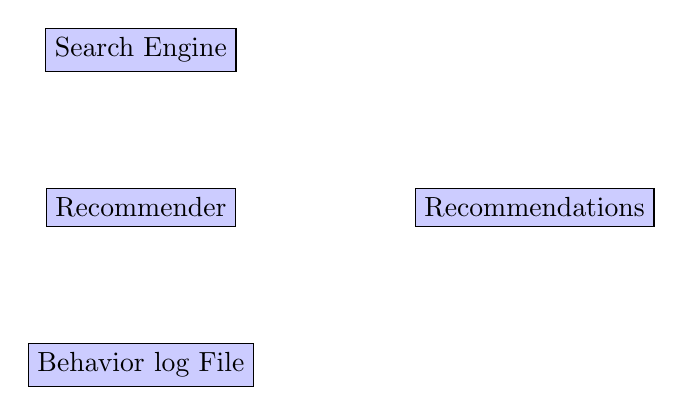
\begin{tikzpicture}[node distance=20mm,
data/.style={
rectangle,
draw,
thin,
fill=blue!20
}]
\node (recommender) [data] {Recommender};
\node (topn) [data,right of = recommender, node distance=50mm] {Recommendations};
\node (history) [data,below of = recommender] {Behavior log File};
\node (db) [data,above of= recommender] {Search Engine};
\end{tikzpicture}
\caption{Recommender engine}
\end{figure}

\section{Sample Input Data}
\label{sec:sampleinput}

\begin{lstlisting}[label=lst:sampledata]
itemid, userid, timestamp
1,101,980730861
1,102,980731380
1,103,980731926
2,101,980732037
2,103,980730408
2,104,980731766
3,101,980731282
3,102,980730769
3,103,980731208
4,102,980732235
4,103,980731417
5,101,980731745
5,102,980731621
5,103,980731417
5,104,980731208  
\end{lstlisting}

\section{Case Study: artoffer.ch}
\label{sec:artoffer}

The following action are used as indicators
\begin{itemize}
\item When a user visits the page of a item. (boolean)
\item When a user likes an item.
\item Tags
\end{itemize}
